\section{Intégrale de \textsc{Poisson} : une utilisation des sommes de \textsc{Riemann}}

\todoinline{Pourrait-on trouver le contexte où cette intégrale apparaît ?}
\todoarmand{
Un dm \url{http://alain.troesch.free.fr/2023/Fichiers/dm11.pdf} qui montre comment le calcul de cette intégrale peut se ramener à
l’intégrale du noyau de Poisson.
}

%---------------

\begin{prop}
Pour tout $x \in \R_+$, on pose $I(x) = \int_0^\pi \ln(1 - 2 x \cos t + x^2) \d t$. Alors, pour tout $x$ réel positif,
\begin{align*}
I(x) &= 2 \pi \ln(x).
\end{align*}
\end{prop}


\begin{exercice}[Intégrale de \cite{Poisson}]
\begin{questions}
\item Montrer que $I$ est bien définie sur $\R_+$.

\item Soit $n \in \N^\star$ et $x \neq 1$. Déterminer une expression simple de $\sum_{k=0}^{n-1} \ln\left(1 - 2 x \cos\left(\frac{k\pi}{n}\right) + x^2\right)$.

\item En déduire la valeur de $I(x)$ pour $x \neq 1$.

\item Montrer que $I(1) = 2 \pi\ln(2) + 4 \int_0^{\pi/2} \ln(\sin(u)) \d u$.

\item En déduire la valeur de $I(1)$.
\end{questions}
\end{exercice}


\begin{solution}
\begin{reponses}
\item En utilisant le discriminant réduit, $\cos^2(t) - 1 < 0$ sur $]0,\pi[$ donc le trinôme n'admet pas de racine et le logarithme est bien défini.

De plus, en $t = 0$, $1 - 2 x + x^2 = (1 - x)^2 > 0$ car $x \neq 1$.

En $t = \pi$, $1 + 2 x + x^2 = (1 + x)^2 > 0$ car $x \neq 1$.

Ainsi, $I(x)$ est bien définie pour $x \neq 1$.

\item En utilisant les factorisations classiques ainsi que les résultats sur les racines $n$-èmes de l'unité,
\begin{align*}
\prod_{k=0}^{n-1} \left(1 - 2 \cos\left(\frac{k\pi}{n}\right) x + x^2\right)
&= \prod_{k=0}^{n-1} \left(x - \e^{ik\pi/n}\right) \left(x - \e^{-ik\pi/n}\right) \\
&= \prod_{k=0}^{n-1} \left(x - \e^{2ik\pi/(2n)}\right) \prod_{k=n+1}^{2n} \left(x - \e^{2ik\pi/(2n)}\right) \\
&= \frac{x^{2n} - 1}{x + 1} (x - 1)
\end{align*}
\item D'après les calculs précédents, et en utilisant une somme de Riemann de pas $\frac{\pi}{2n}$,
\begin{align*}
S_n(f) &= \frac{\pi}{2n} \ln\abs{x^{2n}-1} - \frac{\pi}{n} \ln \abs{\frac{x+1}{x-1}} \\
&= 2 \pi \ln\abs{x} + \frac{\pi}{n} \ln \abs{1 - x^{-2n}} - \frac{\pi}{n} \ln \abs{\frac{x+1}{x-1}}.
\end{align*}

Ainsi, $\lim_{x\to +\infty} S_n(f) = 2 \pi \ln\abs{x}$.

Finalement, pour tout $x \neq 1$, $I(x) = 2 \pi \ln\abs{x}$.
\item D'après les propriétés des fonctions trigonométriques,
\begin{align*}
\ln(2 - 2 \cos(t)) &= \ln(2(1 - \cos(t))) \\
&= \ln(4 \sin^2(t/2)) \\
&= \ln(4) + 2 \ln(\sin(t/2))
\end{align*}

\item En effectuant le changement de variable $\phi : u \mapsto 2 u$,
\begin{align*}
\int_0^\pi \ln(2 - 2 \cos(t)) \d t &= 2 \pi \ln(2) + 2 \int_0^\pi \ln(\sin(t/2)) \d t \\
&= 2 \pi \ln(2) + 4 \int_0^{\pi/2} \ln(\sin(u)) \d u
\end{align*}
Or, $\int_0^{\pi/2} \ln(\sin(u)) \d u = \int_0^{\pi/2} \ln(\cos(u)) \d u$. Ainsi,
% \begin{comment}

\begin{align*}
\int_0^{\pi/2} \ln(\sin(u)) \d u + \int_0^{\pi/2} \ln(\cos(u)) \d u
&= \int_0^{\pi/2} \ln(\sin(2 t)) \d t - \frac{\pi}{2} \ln(2) \\
&= \frac{1}{2} \int_0^\pi \ln(\sin t)) \d t - \frac{\pi}{2} \ln(2) \\
&= \frac{1}{2} \int_0^{\pi/2} \ln(\sin t)) \d t\\
&\qquad + \frac{1}{2} \int_{\pi/2}^{\pi} \ln(\sin t)) \d t - \frac{\pi}{2} \ln(2) \\
&= \int_0^{\pi/2} \ln(\sin t) \d t - \frac{\pi}{2} \ln(2)
\end{align*}

Ainsi,
\[
\int_0^{\pi/2} \ln(\sin(t)) \d t = -\frac{\pi}{2} \ln(2)
\]

D'où $I(1) = 0$.
% \end{comment}
\end{reponses}
\end{solution}

\begin{marginfigure}[-5cm]
    \centering
    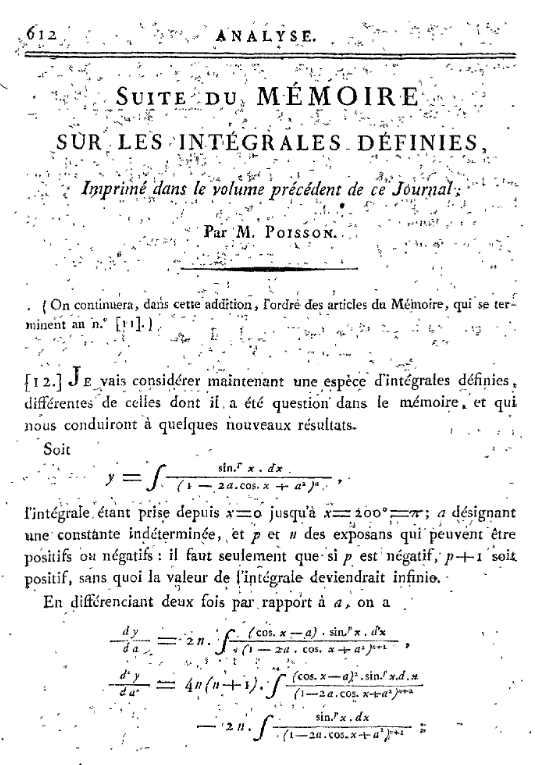
\includegraphics[scale=0.08]{illustrations/Journal_de_l_ecole_polytechnique_cahier_17_1815.png}
    % 
\includepdf[pages={3},scale=.4]{Journal_de_l_ecole_polytechnique_cahier_17_1815.pdf}
    % \caption{\chevron{Suite du mémoire sur les intégrales définies}, Journal de l'École polytechnique, Cahier 17, X (1815), 612-631 (% \url{https://gallica.bnf.fr/ark:/12148/bpt6k433673r/f614.item})}
\end{marginfigure}
\todoarmand{Problème avec la légende de la figure}
